% Theorie: Physikalische Grundlagen von Versuch/Messverfahren, Gleichungen ohne Herleitung knapp erklären
\section[Theorie]{Theorie \textnormal{\cite{paramagnet}}}
\label{sec:theorie}

\subsection{Magnetismus und Materie}

Der im Vakuum geltende Zusammenhang zwischen magnetischer Flussdichte $\symbf B$ und magnetischer Feldstärke $\symbf H$
\begin{equation*}
	\symbf B = \mu_0 \symbf H
	\label{eqn:vakuum}
\end{equation*}
muss unter Anwesenheit von Materie um die Magnetisierung $\symbf M$ zu
\begin{equation*}
	\symbf B = \mu_0 \symbf H + \symbf M
	\label{eqn:materie}
\end{equation*}
ergänzt werden. Dabei beschreibt $\mu_0$ die magnetische Feldkonstante. Verantwortlich für das Auftreten von $\symbf M$
sind atomare magnetische Momente im betrachteten Material. Daher lässt sich die Magnetisierung mit dem mittleren
magnetischen Moment $\bar{\symbf \mu}$ und der Anzahl der Momente pro Volumen $N$ als
\begin{equation}
	\symbf M = N \mu_0 \, \bar{\symbf \mu}
	\label{eqn:magnet_moment}
\end{equation}
ausdrücken. Ihre Abhängigkeit zu $\symbf H$ wird über
\begin{equation}
	\symbf M = \mu_0 \, \chi \symbf H
	\label{eqn:magnet_feld}
\end{equation}
formuliert. Der Faktor $\chi$ heißt magnetische Suszeptibilität und weist selbst komplexe Beziehungen zur Feldstärke
$\symbf H$ und Temperatur $T$ auf.

\subsubsection{Diamagnetismus}

Durch die Induktion magnetischer Momente beim Einwirken äußerer Magnetfelder tritt in allen Atomen das Phänomen des
Diamagnetismus auf. Das induzierte Feld ist dem ursächlichen dabei entgegengesetzt und schwächt so dessen Einfluss ab.
Für die Suszeptibilität muss dann $\chi < 0 $ gelten. Ideale Diamagneten werden durch Supraleiter realisiert, welche
$\chi = -1$ erreichen und das Magnetfeld in ihrem Inneren vollständig verdrängen.

\subsubsection{Paramagnetismus}

Anders als der Diamagnetismus ist der Paramagnetismus keine universelle Eigenschaft der Materie, sondern lässt sich nur
bei Atomen, Ionen und Molekülen beobachten, deren Gesamtdrehimpuls nicht verschwindet. Bei Abwesenheit eines äußeren
Feldes sind die an den Drehimpuls gekoppelten magnetischen Momente durch thermische Bewegung zufällig orientiert, sodass
keine mittlere Magnetisierung existiert. Wird jedoch ein Magnetfeld angelegt, richten sich die Momente parallel dazu aus,
sodass dessen Wirkung verstärkt wird. Die Suszeptibilität erfüllt dann $\chi > 0$ und ist aufgrund des Störeinflusses der
thermischen Bewegung temperaturabhängig. Anhand dieses Modells kann $\chi$ nun berechnet werden.

\subsection{Paramagnetische Suszeptibilität} 

Der atomare Gesamtdrehimpuls $\symbf J$ setzt sich aus Bahndrehimpuls der Elektronenhülle und Eigendrehimpuls der
Elektronen, dem Spin, zusammen. Für den Paramagnetismus kann der Beitrag des zusätzlich auftretenden Kerndrehimpulses
vernachlässigt werden. Solange das äußere Magnetfeld nicht zu stark ist, wird von LS-Kopplung mit
\begin{equation*}
	\symbf J = \symbf L + \symbf S
	\label{eqn:kopplung}
\end{equation*}
ausgegangen, also der Annahme, dass $\symbf J$ der Vektorsumme von Gesamtbahndrehimpuls~$\symbf L$ und Gesamtspin
$\symbf S$ entspricht. Dabei setzen sich $\symbf L$ und $\symbf S$ nach
\begin{align*}
	\symbf L = \sum_i \symbf l_i && \symbf S = \sum_i \symbf s_i
\end{align*}
aus der jeweiligen Vektorsumme der Einzeldrehimpulse sämtlicher in der Hülle enthaltenen Elektronen zusammen. Anwenden
quantenmechanischer Mittel liefert dann die zugehörigen magnetischen Momente, welche sich auf
\begin{align}
	\symbf \mu_L &= - \frac{\mu_B}{\hbar} \symbf L \label{eqn:mu_L}
	\shortintertext{und}
	\symbf \mu_S &= - g_s \frac{\mu_B}{\hbar} \symbf S \label{eqn:mu_S}
\end{align}
belaufen. Dabei entspricht $\hbar = \frac{h}{2\pi}$ der reduzierten Planck-Konstante, die mit Wirkungsquantum $h$,
Frequenz $\nu$ und Kreisfrequenz $\omega$ die Beziehung $h \nu = \hbar \omega$ erfüllt. Mit der Ladung $e_0$ und
Ruhemasse $m_0$ des Elektrons bezeichnet das Bohrsche Magneton
\begin{equation*}
	\mu_B = \frac{1}{2} \frac{e_0}{m_0} \hbar
	\label{eqn:magneton}
\end{equation*}
das zur Drehimpulseinheit $\hbar$ gehörige magnetische Moment. Ebenso ist mit der negativen Ladung des Elektrons das
negative Vorzeichen in \eqref{eqn:mu_L} und \eqref{eqn:mu_S} erklärt. Der Faktor $g_S$ entspricht dem gyromagnetischen
Verhältnis des freien Elektrons.

Unter Verwendung der Bahndrehimpulsquantenzahl $L$, Spinquantenzahl $S$ und Gesamtdrehimpulsquantenzahl $J$ des Atoms lässt sich
\begin{align}
	| \symbf L | = \sqrt{L(L+1)} \hbar &&
	| \symbf S | = \sqrt{S(S+1)} \hbar &&
	| \symbf J | = \sqrt{J(J+1)} \hbar \label{eqn:abs}
\end{align}
für die Beträge der Drehimpulse schreiben. Aus \eqref{eqn:mu_L} und \eqref{eqn:mu_S} folgt damit weiter
\begin{align}
	| \symbf \mu_L | &= \frac{\mu_B}{\hbar} | \symbf L | = \mu_B \sqrt{L(L+1)} \label{eqn:abs_mu_L}
	\shortintertext{und}
	| \symbf \mu_S | &= g_s \frac{\mu_B}{\hbar} | \symbf S | = g_S \, \mu_B \sqrt{S(S+1)} \label{eqn:abs_mu_S}
\end{align}
für die entsprechenden magnetischen Momente. Bei LS-Kopplung verschwindet die zu $\symbf J$ orthogonale Komponente von $\symbf \mu$,
sodass nur $\symbf \mu_J \parallel \symbf J$ messbar ist. In Abbildung \ref{fig:diagramm} kann dazu der Zusammenhang
\begin{equation}
	| \symbf \mu_J | = | \symbf \mu_S | \cos \alpha + | \symbf \mu_L | \cos \beta
	\label{eqn:abs_mu_J}
\end{equation}
abgelesen werden. Zudem lässt sich nach dem Cosinussatz mittels des Dreiecks $OAB$
\begin{align}
	\cos \alpha = \frac{ | \symbf J |^2 - | \symbf L |^2 + | \symbf S |^2 }{2| \symbf J || \symbf S |} &&
	\cos \beta = \frac{ | \symbf J |^2 + | \symbf L |^2 - | \symbf S |^2 }{2| \symbf J || \symbf S |}
	\label{eqn:cosine}
\end{align}
aus Abbildung \ref{fig:diagramm} herleiten.

\begin{figure}[H]
	\centering
	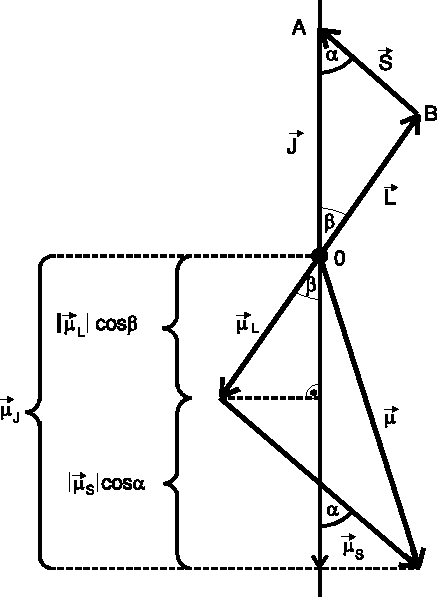
\includegraphics{content/grafik/diagramm.pdf}
	\caption{Vektordiagramm der Drehimpulse einer Elektronenhülle mit den resultierenden magnetischen Momenten.}
	\label{fig:diagramm}
\end{figure}

Einsetzen von \eqref{eqn:abs}, \eqref{eqn:abs_mu_L}, \eqref{eqn:abs_mu_S} und \eqref{eqn:cosine} in die Beziehung
\eqref{eqn:abs_mu_J} liefert nun
\begin{align*}
	| \symbf \mu_J | &= \mu_B \left( g_S \sqrt{S(S+1)} \cos \alpha + \sqrt{L(L+1)} \cos \beta \right) \\
	&= \mu_B \frac{(g_S + 1)J(J+1) + (g_S - 1) \left( S(S+1) - L(L+1) \right) }{2\sqrt{J(J+1)}}
\end{align*}
als Betrag des magnetischen Moments. Anhand der Größe $g_S$ kann mit guter Genauigkeit die Näherung $g_S \approx 2$ ausgenutzt werden,
um über den für das Atom spezifischen Landé-Faktor
\begin{equation}
	g_J = \frac{3J(J+1) + \left( S(S+1) - L(L+1) \right)}{2J(J+1)}
	\label{eqn:lande}
\end{equation}
den Ausdruck
\begin{equation}
	| \symbf \mu_J | \approx \mu_B \, g_J \sqrt{J(J+1)}
	\label{eqn:approx_abs_mu_J}
\end{equation}
zusammenzufassen. Ein weiteres quantenmechanisches Phänomen ist die Richtungsquantelung, wonach der Winkel zwischen einem äußeren
Magnetfeld und $\symbf \mu_J$ nicht beliebig ist, sondern nur solche Werte einnimmt, bei denen die Komponente $\mu_{J_z}$ von
$\symbf \mu_J$ in Feldrichtung ein ganzzahliges Vielfaches von $\mu_B g_J$ darstellt. Entsprechend muss
\begin{equation*}
	\mu_{J_z} = - \mu_B \, g_J \, m
	\label{eqn:komponente}
\end{equation*}
gelten, wobei $m \in \symbb{Z}$ die Orientierungsquantenzahl bezeichnet. Da $\mu_{J_z}$ als Komponente von $\symbf \mu_J$ immer
$| \mu_{J_z} | \leq | \symbf \mu_J |$, also laut \eqref{eqn:approx_abs_mu_J} $m \leq \sqrt{J(J+1)}$ erfüllt, führt die Einschränkung
$m \in \{ -J, -J+1, \dotsc, 0, \dotsc, J-1, J \}$ zu dem Schluss, dass genau $2J+1$ Möglichkeiten zur Einstellung des magnetischen
Moments relativ zur äußeren Feldrichtung existieren. Jeder dieser Einstellrichtungen lässt sich eine spezifische potentielle
Energie
\begin{equation*}
	E_m = - \symbf \mu_J \cdot \symbf B = \mu_{J_z} B = \mu_B \, g_J \, m B
	\label{eqn:zeeman}
\end{equation*}
zuordnen. Dieses Auftreten von $2J+1$ Unterenergieniveaus heißt Zeeman-Effekt. Deren Besetzungshäufigkeit folgt mit
\begin{equation*}
	Z(E_m,T) = \exp \! \left( - \pfrac{E_m}{kT \,} \right)
	\label{eqn:boltzmann}
\end{equation*}
einer Boltzmann-Verteilung, Summation über alle Niveaus liefert
\begin{equation*}
	\mu_\text{ges} = \sum_{m = -J}^J -\mu_B \, g_J \, m Z(E,T) = -\mu_B \, g_J
	\sum_{m = -J}^J m \, \exp \! \left( - \frac{\mu_B \, g_J \, mB}{kT \,} \right)
	\label{eqn:mu_ges}
\end{equation*}
für das gesamte magnetische Moment.
\newpage
Nach Division durch die Gesamthäufigkeit aller vorkommenden Orientierungen ergibt sich daraus
\begin{equation}
	\bar{\mu} = - \mu_B \, g_J \, \frac{\displaystyle{\sum_{m = -J}^J m \, \exp \! \left( - \frac{\mu_B \, g_J \, mB}{kT \,} \right)}}
	{\displaystyle{\sum_{m = -J}^J \exp \! \left( - \frac{\mu_B \, g_J \, mB}{kT \,} \right)}}
	\label{eqn:mu_mittel}
\end{equation}
als Betrag des in \eqref{eqn:magnet_moment} geforderten mittleren magnetischen Moments. Der Quotient in Ausdruck~\eqref{eqn:mu_mittel}
wird als Brillouin-Funktion bezeichnet. Bei einer Temperatur im Bereich $T \approx \qty{300}{\kelvin}$ sowie unter Einwirkung von
Flussdichten bis $B \approx \qty{1}{\tesla}$ gilt
\begin{equation*}
	\frac{\mu_B \, g_J \, mB}{kT} \ll 1
	\label{eqn:kleiner}
\end{equation*}
und erlaubt mit der Entwicklung
\begin{equation*}
	\exp \! \left( - \frac{\mu_B \, g_J \, mB}{kT \,} \right) \simeq 1 - \frac{\mu_B \, g_J \, mB}{kT \,}
	\label{eqn:naeherung}
\end{equation*}
das Aufstellen einer Näherungsformel. So ergibt sich
\begin{equation}
	\sum_{m = -J}^J \left( 1 - \frac{\mu_B \, g_J \, mB}{kT \,} \right) =
	2J + 1 - \frac{\mu_B \, g_J \, B}{kT \,} \sum_{m = -J}^J m = 2J + 1
	\label{eqn:nenner}
\end{equation}
für den Nenner der Funktion, der Zähler ist mit
\begin{equation}
	\sum_{m = -J}^J \left( m - \frac{\mu_B \, g_J \, m^2 B}{kT \,} \right) =
	- \frac{\mu_B \, g_J \, B}{kT \,} \sum_{m = -J}^J m^2 =
	- \frac{\mu_B \, g_J \, B}{3kT \,} J(J+1)(2J+1)
	\label{eqn:zaehler}
\end{equation}
gegeben. Einsetzen von \eqref{eqn:mu_mittel}, \eqref{eqn:nenner} und \eqref{eqn:zaehler} in Gleichung \eqref{eqn:magnet_moment}
liefert den Term
\begin{equation*}
	M = N \mu_0 \, \bar{\mu} = N \mu_0 \, \mu_B^2 \, g_J^2 \, \frac{J(J+1)B}{3kT}
	\label{eqn:magnet_betrag}
\end{equation*}
als Betrag der makroskopischen Magnetisierung. Aus der Äquivalenz \eqref{eqn:magnet_feld} folgt dann mit
\begin{equation}
	\chi = \frac{N \mu_0 \, \mu_B^2 \, g_J^2 \, J(J+1)}{3kT}
	\label{eqn:chi_theo}
\end{equation}
die magnetische Suszeptibilität, welche damit dem Zusammenhang
\begin{equation*}
	\chi \sim \pfrac{1}{T\,}
	\label{eqn:curie}
\end{equation*}
gehorcht. Dabei handelt es sich um das Curiesche Gesetz des Paramagnetismus, dessen Gültigkeit
hiermit für ausreichend hohe Temperaturen belegt ist.

\subsubsection{Seltene-Erd-Verbindungen}

Aus der experimentellen Erkenntnis, dass Verbindungen, die Ionen Seltener Erden enthalten, stark paramagnetisch sind, lässt sich
unter Betrachtung von Formel~\eqref{eqn:chi_theo} auf die Existenz großer Drehimpulse in den Elektronenhüllen Seltener-Erd-Atome
schließen. Dabei muss es sich zudem um innere Elektronen handeln, um den Paramagnetismus auch im ionisierten Zustand zu erklären.
Alle Elemente der Seltenen Erden besitzen mit der vollständigen \ce{Xe}-Hülle Elektronen bis zur 5p- sowie zwei weitere in der
6s-Schale. Diese sind in der weiteren Betrachtung jedoch nicht relevant, da sämtliche Spins und Bahndrehimpulse gesättigt sind.
Es entsteht so kein von Null verschiedener Gesamtdrehimpuls. Vielmehr sind dafür die tiefer befindlichen 4f-Elektronen
verantwortlich, deren Anordnung den Hundschen Regeln unterliegt:
\begin{enumerate}
	\item Einzelne Spins $\symbf s_i$ sind so kombiniert, dass sie den maximalen mit dem Pauli-Prinzip vereinbaren Gesamtspin
			$\symbf S = \sum_i \symbf s_i$ erreichen, sich also möglichst parallel ausrichten. Nach dem Pauli-Prinzip dürfen
			zwei Elektronen nie in all ihren Quantenzahlen übereinstimmen.
	\item Individuelle Bahndrehimpulse $\symbf l_i$ setzen sich so zusammen, dass immer der maximale Gesamtbahndrehimpuls
			$\symbf L = \sum_i \symbf l_i$ auftritt, welcher sowohl mit dem Pauli-Prinzip als auch der 1. Hundschen Regel verträglich ist.
	\item Ist die Schale weniger als halbvoll, tritt ein Gesamtdrehimpuls $\symbf J = \symbf L - \symbf S$ auf. Ist sie mehr als zur
			Hälfte gefüllt, so ist $\symbf J = \symbf L + \symbf S$ gegeben. Sind genau halb so viele Elektronen wie maximal
			möglich vorhanden, folgt $\symbf L = 0$ aus der 2. Hundschen Regel, sodass immer $J = S$ gilt.	
\end{enumerate}
Basierend auf der gegenseitigen elektrostatischen Abstoßung der Hüllenelektronen finden die Hundschen Regeln im Folgenden zur
Berechnung der magnetischen Suszeptibilität Anwendung, indem aus ihnen Gesamtdrehimpuls $J$ und Landé-Faktor $g_J$ ermittelt werden.
Speziell im Bezug auf die zu betrachtende 4f-Schale gelten einige Einschränkungen. Als f-Schale ist jeder einzelne Bahndrehimpuls
mit $l_i \leq 3$ beschränkt. Daraus folgt weiter eine vollständige Belegung mit einer maximalen Anzahl von 14 Elektronen.

\subsection{Messverfahren}

\subsubsection{Apparatur zur Induktivitätsmessung}

Die Induktivität einer langen Zylinderspule mit Windungszahl $n$, Querschnittsfläche $F$ und Länge $l$ wird über
\begin{equation}
	L = \mu_0 \pfrac{n^2}{\! l} F
	\label{eqn:spule_vak}
\end{equation}
beschrieben. Ist ihr Inneres gänzlich mit Materie gefüllt, gilt
\begin{equation*}
	L_{\widehat{M}} = \mu \, \mu_0 \pfrac{n^2}{\! l} F
	\label{eqn:spule_mat}
\end{equation*}
mit der Permeabilitätszahl $\mu$ als materialspezifischer Skalierungsfaktor.
\enlargethispage*{\baselineskip}
\newpage
Für einen Probenquerschnitt $Q < F$ muss eine Korrektur
\begin{equation*}
	L_M = \mu_0 \pfrac{n^2}{\! l} F + (\mu - 1) \mu_0 \pfrac{n^2}{\! l} Q =
	\mu_0 \pfrac{n^2}{\! l} F + \chi \mu_0 \pfrac{n^2}{\! l} Q = L + \increment L
	\label{eqn:spule_real}
\end{equation*}
vorgenommen werden. Hierbei wird die Induktivitätsänderung
\begin{equation}
	\increment L = \chi \mu_0 \pfrac{n^2}{\! l} Q
	\label{eqn:diff_real}
\end{equation}
eingeführt. Diese fällt im Allgemeinen sehr gering aus, sodass es einer präzisen Messung bedarf. Diesem Zweck dient die in
Abbildung \ref{fig:schaltung} dargestellte Brückenschaltung.

\begin{figure}[H]
	\centering
	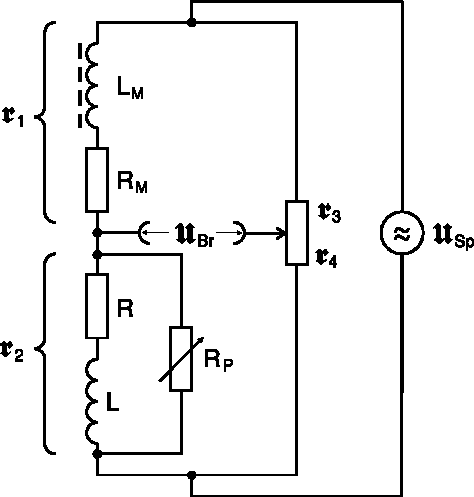
\includegraphics{content/grafik/schaltung.pdf}
	\caption{Brückenschaltung zur präzisen Suszeptibilitätsmessung.}
	\label{fig:schaltung}
\end{figure}

Brückenspannung $\symbffrak U_\text{Br}$ und Speisespannung $\symbffrak U_\text{Sp}$ sind dabei über die Relation
\begin{equation}
	\symbffrak{ U_\text{Br} = \frac{r_4 r_1 - r_3 r_2}{(r_1 + r_2)(r_3 + r_4)} \, U_\text{Sp} }
	\label{eqn:bruecke_gen}
\end{equation}
miteinander verknüpft \cite{brücke}. Dazu lassen sich die komplexen Impedanzen
\begin{align*}
	\symbffrak r_1 = R_M + \symbffrak i \, \omega L_M &&
	\pfrac{1}{\symbffrak r_2} = \pfrac{1}{R_P} + \pfrac{1}{R + \symbffrak i \, \omega L} &&
	\symbffrak r_3 = R_3 && \symbffrak r_4 = R_4
\end{align*}
mit der imaginären Einheit $\symbffrak i$ aufstellen, mit $\omega$ ist die angelegte Spannungsfrequenz bezeichnet.
Um kleinste Unterschiede zwischen den Verlustwiderständen $R$ und $R_M$ der beiden idealerweise identischen Spulen
zu kompensieren, wird der Regelwiderstand $R_P$ verbaut. Für diesen kann $R_P \gg R, \omega L$ angenommen werden, sodass
$\symbffrak r_2 \approx R + \symbffrak i \, \omega L$ gilt.

Aus \eqref{eqn:bruecke_gen} folgt, dass die Abgleichbedingung der Schaltung
\begin{equation}
	\symbffrak r_1 R_4 = \symbffrak r_2 R_3
	\label{eqn:abgleich_ohne}
\end{equation}
ohne Probe für $R_3 \approx R_4$ erfüllt ist. Mit eingebauter Probe wird bei
\begin{equation*}
	R'_3 = R_3 + \increment R
	\label{eqn:R_3}
\end{equation*}
ein neuer Abgleichpunkt gefunden, wegen $R_3 + R_4 = R'_3 + R'_4 = \text{const}$ folgt
\begin{equation*}
	R'_4 = R_4 - \increment R \approx R_3 - \increment R
	\label{eqn:R_4}
\end{equation*}
als Resultat der Implementierung von $R_3$ und $R_4$ als Potentiometer. Durch Einsetzen der neuen Impedanzen folgt aus
\eqref{eqn:abgleich_ohne} die Gleichung
\begin{equation}
	(R_M + \symbffrak i \, \omega L_M)(R_3 - \increment R) = (R + \symbffrak i \, \omega L)(R_3 + \increment R)
	\label{eqn:abgleich_mit}
\end{equation}
als Abgleichbedingung mit durch die Probe veränderter Induktivität. Ihr Imaginärteil lässt sich zu
\begin{equation*}
	\increment R = \frac{R_3 (L_M - L)}{L_M + L}
	\label{eqn:R_delta_1}
\end{equation*}
umformulieren. Einsetzen von $L_M = L + \increment L$ mit der Annahme $\increment L \ll L$ liefert
\begin{equation*}
	\increment R = \frac{R_3 (\increment L)}{2L + \increment L} \approx \frac{R_3 (\increment L)}{2L} 
	\label{eqn:R_delta_2}
\end{equation*}
und weiter mit \eqref{eqn:spule_vak} sowie \eqref{eqn:diff_real} die Formel
\begin{equation*}
	\increment R = \chi \frac{R_3}{2} \frac{Q}{\! F} 
	\label{eqn:R_delta_3}
\end{equation*}
für die notwendige Widerstandsänderung, aus der sich nun
\begin{equation}
	\chi =  2 \pfrac{\increment R}{R_3} \pfrac{F}{Q} 
	\label{eqn:chi_exp}
\end{equation}
zur experimentellen Bestimmung der magnetischen Suszeptibilität ergibt.


\subsubsection{Unterdrückung von Störspannungen}

Die Brückenspannung $\symbffrak U_\text{Br}$ fällt bei der Messung so gering aus, dass sie fast völlig durch das unvermeidbar
auftretende Störrauschen verdeckt wird. Da es sich jedoch um eine monofrequente Signalspannung handelt, ist ein digitaler
Filter durch Sperren aller von der Signalfrequenz $\nu$ verschiedenen Frequenzen in der Lage, die Hintergrundspannungen
zu kompensieren. Ein solches Gerät wird annähernd durch einen Selektivverstärker realisiert, der im wesentlichen aus einem
Bandpass mit Durchlassfrequenz $\nu_0$ besteht. In Abbildung~\ref{fig:kurve} ist ein exemplarischer Verlauf der Ausgangs-
zur Eingangsspannung dargestellt.

\begin{figure}[H]
	\centering
	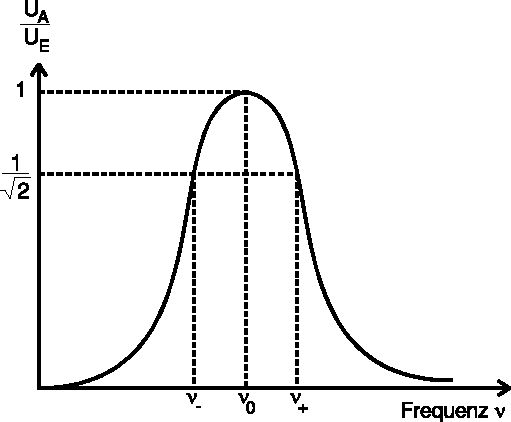
\includegraphics{content/grafik/kurve.pdf}
	\caption{Filterkurve zu Güte und Funktion eines Selektivverstärkers.}
	\label{fig:kurve}
\end{figure}

Es ist zu erkennen, dass für $\nu = \nu_0$ im angrenzenden Frequenzbereich nicht alle Störspannungen unterdrückt sind. Ein Maß für
die Breite dieser Region ist durch die Güte
\begin{equation*}
	Q = \frac{\nu_0}{\nu_+ - \nu_-}
	\label{eqn:gut}
\end{equation*}
gegeben. Das Intervall $\mathopen[ \nu_-, \nu_+ \mathclose]$ enthält hier solche Frequenzen, die
$\sqrt{2} \, U_{\! A} \geq U_E$ erfüllen.
